%%%%%%%%%%%%%%%%%%%%%%%%%%%%%%%%%%%%%%%%%%%%%%%%%%%%%%%%%%
% "How to use the Spaceprobe"
%
% https://github.com/makehackvoid/spaceprobe
%
% Adapted from "A Template for 'How to create a WiFi account' with Re2o'"
% https://github.com/Klafyvel/create_account_re2o_poster
% Images belong to their authors
%
% Distributed under Creative Commons CC BY 4.0
%%%%%%%%%%%%%%%%%%%%%%%%%%%%%%%%%%%%%%%%%%%%%%%%%%%%%%%%%%


% Here you can set the color and the text size
% Rézo Metz : 1cc0fa
% Aurore : cf0f23
\documentclass[color=1cc0fa, size=12pt, logo=mhv-logo.png]{re2o-poster}

\newcommand{\intranet}[1]{\newcommand{\theintranet}{#1}\newcommand{\thecontact}{#1/contact/}}
\newcommand{\forum}[1]{\newcommand{\theforum}{#1}}
\newcommand{\github}[1]{\newcommand{\thegithub}{#1}}

% Some informations
\title{How to use the Spaceprobe}
\forum{https://forum.makehackvoid.com}
\github{https://github.com/makehackvoid/spaceprobe}

% You should not need to change anything below

\usepackage[utf8]{inputenc}
\usepackage[T1]{fontenc}

\usepackage{tabularx}
\usepackage{multicol}
\usepackage{qrcode}
\usepackage{cclicenses}
\usepackage{graphicx}

\graphicspath{{images/}}

\begin{document}

\maketitle

\vskip \baselineskip
\begin{minipage}[0.6\pageheight]{\linewidth}
\Large 
\begin{enumerate}

\item Ensure that the meter is at 0
\begin{center}
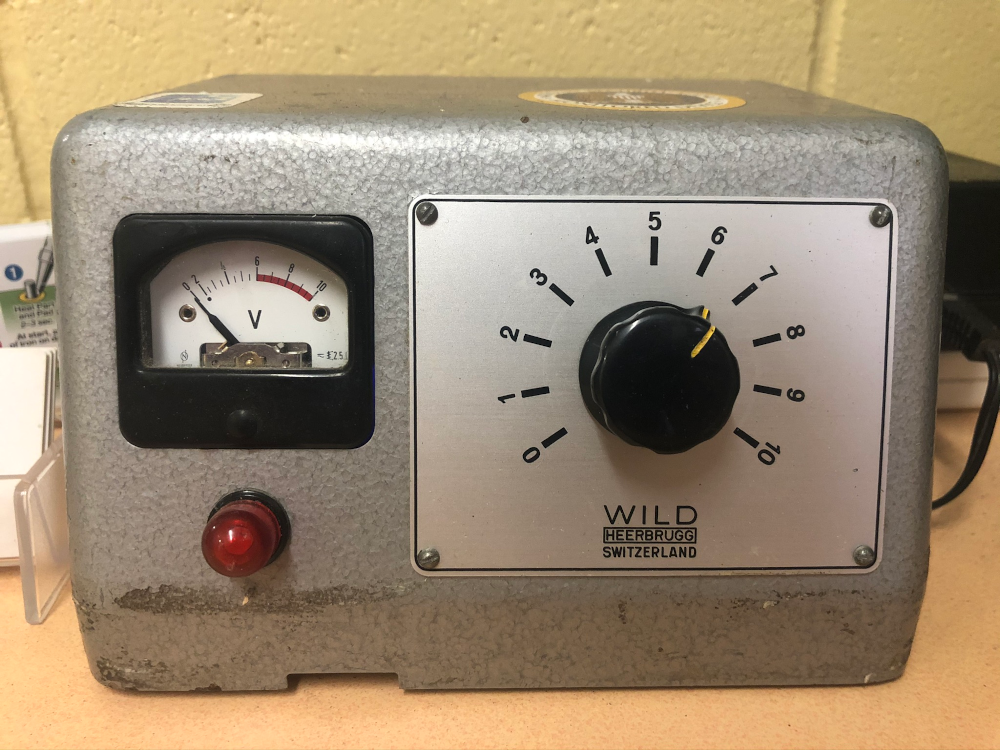
\includegraphics[width=0.4\textwidth]{probe-neutral.png}
\end{center}

\item Turn the knob until the \emph{meter} shows the time you plan to be open for (the knob is on a rotary encoder, so the labels aren't relevant)
\begin{center}
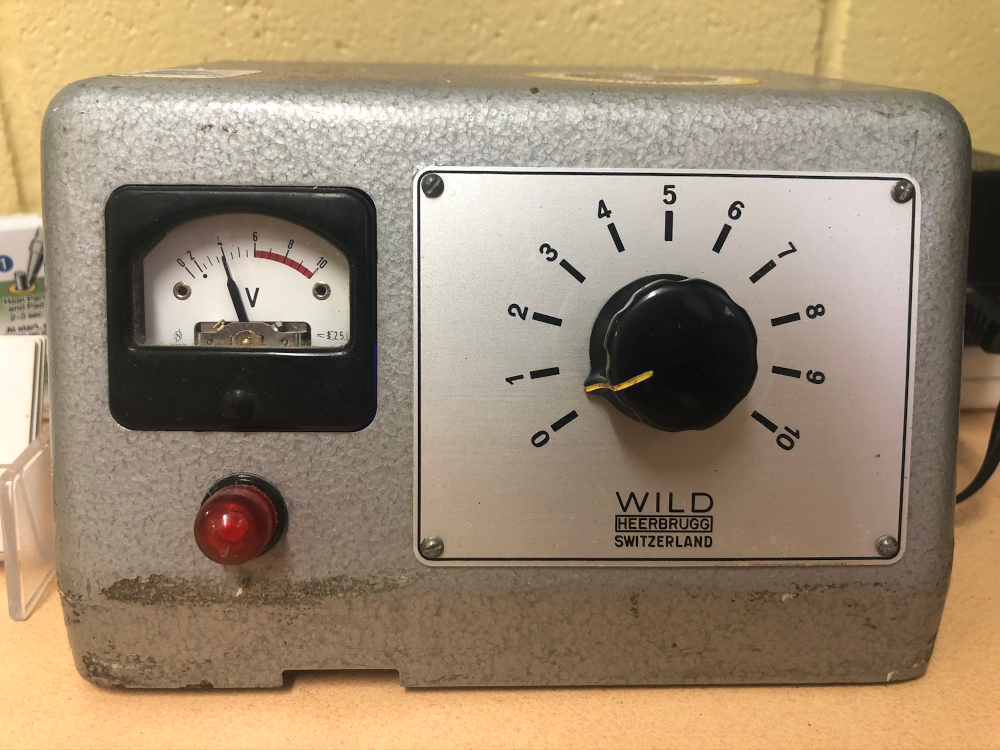
\includegraphics[width=0.4\textwidth]{probe-timeset.png}

The meter shows 4 hours
\end{center}

\item Press the knob in; The LED should flash, and the meter should return to 0

\item Success! The probe should have tweeted
\begin{center}

\includegraphics[width=0.4\textwidth]{tweet.png}
\end{center}


\end{enumerate}
\end{minipage}

\vskip \baselineskip

\hskip -1.1cm%
\renewcommand{\arraystretch}{1.8}%


\vfill
\vskip -0.9\baselineskip
{
\footnotesize
\qrcode[height=0.08\linewidth]{\thegithub} %
\hskip 1cm %
An issue? \emph{\thegithub} %
Or post on the forum \emph{\theforum}
}

\end{document}
